\apendice{Especificación de diseño}

\section{Introducción}
Una vez definidos los requisitos y casos de uso, en este apartado se van a definir las especificaciones de datos para cumplir dichos requisitos.



\section{Diseño de datos}
\subsection{Base de datos}
La base de datos que se eligió para desarrollar el proyecto es \textit{MySql}. La estructura de base de datos se compone de las siguientes tablas:
\begin{itemize}
    \item \textit{\textbf{USERS}}: En esta tabla se almacena toda la información referente a la sesión de los usuarios, se compone de las siguientes columnas:
        \begin{itemize}
            \item\textit{\textbf{user\_id}}: identificador numérico único autoincremental.
            \item \textit{\textbf{active}}: Hace referencia si el usuario está activo en ese momento o no.
            \item \textit{\textbf{username}}: Nombre identificador del usuario.
            \item \textit{\textbf{chat\_id}}: Identificador de \textit{Janus}.
            \item \textit{\textbf{last\_seen}}: Marca temporal de la ultima conexión.
            \item \textit{\textbf{uwb\_id}}: \textit{Foreing key} de las tablas \textit{Tags} y \textit{Tags\_history}, coincidiendo, es el identificador único de la dos tablas.
        \end{itemize}
    \item \textit{\textbf{TAGS}}: Tabla en la que se guarda toda la información referente a los \textit{Tags}.
            \begin{itemize}
                \item \textit{\textbf{tag\_id}}: Identificador único auto incremental.
                \item \textit{\textbf{alias}}: Identificador único enlazado a a la placa \textit{uwb} con la que se guardará.
                \item \textit{\textbf{latitude}}: coordenada de latitud del \textit{tag}.
                \item \textit{\textbf{longitude}}: coordenada de longitud del \textit{tag}.
                \item \textit{\textbf{coordinates}}: geojson en formato punto en forma de \textit{string} con la longitud y la latitud, para la representación.
                \item \textit{\textbf{pos\_x}}: Coordenada local en el eje x.
                \item \textit{\textbf{pos\_y}}: Coordenada local en el eje y.
                \item \textit{\textbf{pos\_z}}: Coordenada local en el eje z.
                \item \textit{\textbf{last\_update}}: Marca temporal con la ultima actualización.
            \end{itemize}
    \item \textit{\textbf{TAGS\_HISTORY}}: Tabla con el histórico de registro de cambios de las \textit{Tags} a tiempo real.
            \begin{itemize}
                \item \textit{\textbf{tag\_id}}: Identificador único auto incremental.
                \item \textit{\textbf{alias}}: Identificador único enlazado a a la placa \textit{uwb} con la que se guardará.
                \item \textit{\textbf{latitude}}: coordenada de latitud del \textit{tag}.
                \item \textit{\textbf{longitude}}: coordenada de longitud del \textit{tag}.
                \item \textit{\textbf{coordinates}}: geojson en formato punto en forma de \textit{string} con la longitud y la latitud, para la representación.
                \item \textit{\textbf{pos\_x}}: Coordenada local en el eje x.
                \item \textit{\textbf{pos\_y}}: Coordenada local en el eje y.
                \item \textit{\textbf{pos\_z}}: Coordenada local en el eje z.
                \item \textit{\textbf{time\_received}}: Marca de temporal de cuando se realizó el cambio.
            \end{itemize}
    \item \textit{\textbf{ANCHORS}}: Tabla que guarda toda la información relacionada con los \textit{anchors}.
            \begin{itemize}
                \item \textit{\textbf{anchor\_id}}: Identificador único auto incremental.
                \item \textit{\textbf{alias}}: Identificador único enlazado a a la placa uwb con la que se guardará.
                \item \textit{\textbf{latitude}}: coordenada de latitud del \textit{anchor}.
                \item \textit{\textbf{longitude}}: coordenada de longitud del \textit{anchor}.
                \item \textit{\textbf{pos\_x}}: Coordenada local en el eje x.
                \item \textit{\textbf{pos\_y}}: Coordenada local en el eje y.
                \item \textit{\textbf{pos\_z}}: Coordenada local en el eje z.
            \end{itemize}
    \item \textit{\textbf{ROOMS}}: Tabla que guarda toda la información básica de las \textit{Rooms}.
            \begin{itemize}
                \item \textit{\textbf{room\_id}}: Identificador numérico único auto incremental de las habitaciones.
                \item \textit{\textbf{alias}}: Identificador en forma de \textit{string} que se le da a una habitación determinada.
                \item \textit{\textbf{coordinates}}: \textit{geojson} tipo \textit{polygon} en formato \textit{string} que incluye las coordenadas del poligono para su representación.
            \end{itemize}
    \item \textit{\textbf{ARTWORK}}: Tabla que guarda toda la información básica de las obras de arte.
            \begin{itemize}
                \item \textit{\textbf{artwork\_id}}: Identificador numérico único auto incremental de las obras de arte.
                \item \textit{\textbf{name}}: Nombre de la obra de arte.
                \item \textit{\textbf{draw}}: coordenadas locales para la representación de el dibujado.
            \end{itemize}
\end{itemize}
\FloatBarrier
\begin{figure}[h]
    \centering
    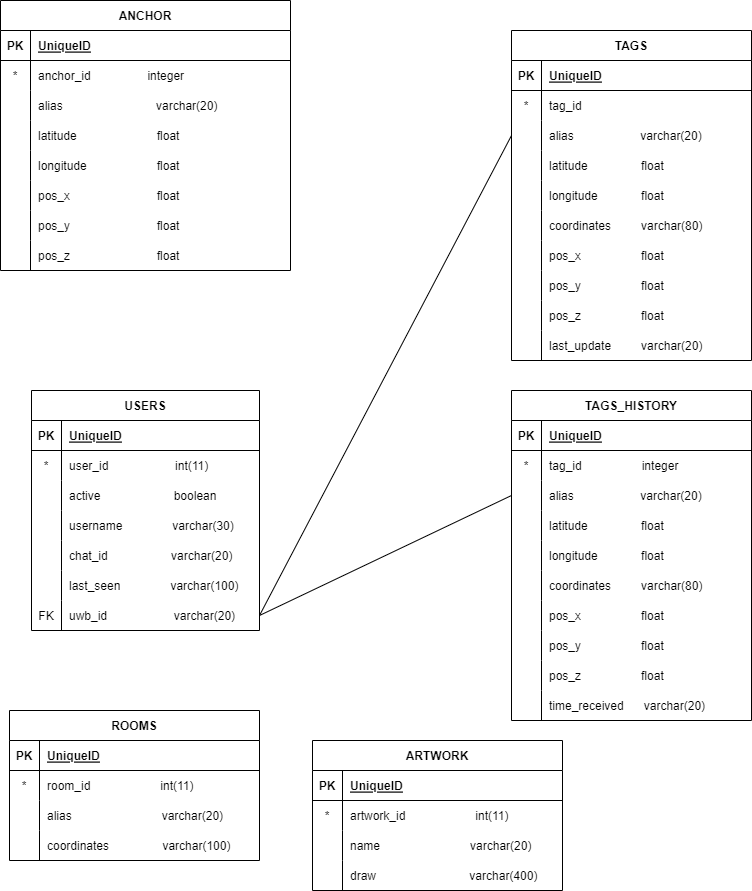
\includegraphics[width=10cm,height=10cm,keepaspectratio]{img/DB COLOSSEUM.drawio.png}
    \caption{Diagrama base de datos.}
    \label{fig:diagram_db}
\end{figure}
\FloatBarrier

\section{Diseño procedimental}
En esta sección se explicará los diagramas de secuencia de una entrada normal a la aplicación web, con todos los sistemas previamente configurados y funcionando.
Para un usuario normal:

\FloatBarrier
\begin{figure}[h]
    \centering
    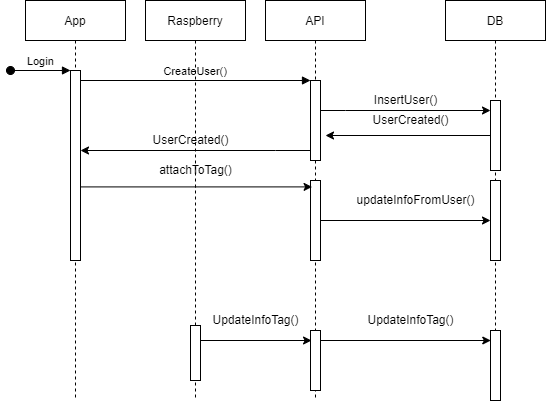
\includegraphics[width=10cm,height=10cm,keepaspectratio]{img/Diagrama procedimental Usuario.drawio (1).png}
    \caption{Diagrama de secuencia de un usuario normal.}
    \label{fig:diagram_seceunce_user}
\end{figure}
\FloatBarrier
Se pueden observar distintas ramas que van hacia la API:
\begin{itemize}
    \item La creación de un usuario en el \textit{login}.
    \item El enlace de un \textit{Tag} a un usuario.
    \item La actualización de la información de posicionamiento desde la \textit{Raspberry}.
\end{itemize}

Se pueden observar que todas las ramas principales utilizan la base de datos.



Para un usuario guía: 
\FloatBarrier
\begin{figure}[h]
    \centering
    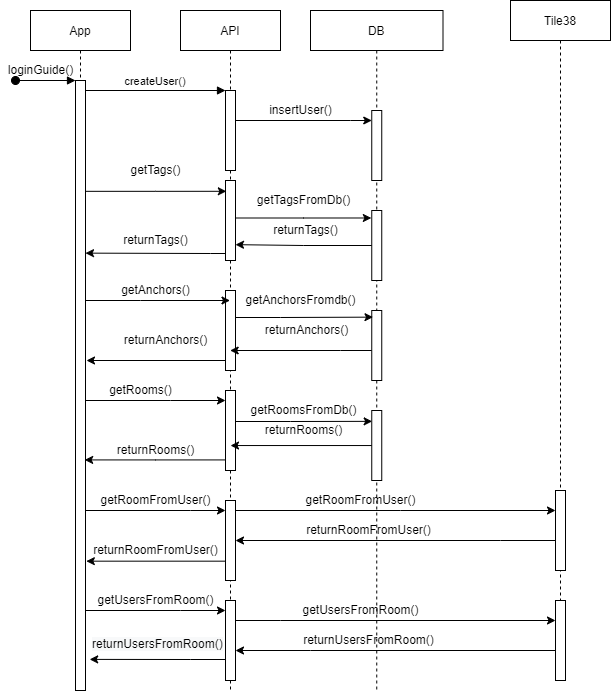
\includegraphics[width=10cm,height=10cm,keepaspectratio]{img/Guide Diagram secuencia.drawio.png}
    \caption{Diagrama de secuencia de un usuario normal.}
    \label{fig:diagram_seceunce_guide}
\end{figure}
\FloatBarrier

Se pueden observar las distintas ramas principales:
\begin{itemize}
    \item La creación de un usuario en el \textit{login}.
    \item La obtención de las \textit{Tags} para mostrarlas en el mapa.
    \item La obtención de los \textit{Anchors} para mostrarlos en el mapa.
    \item La obtención de las \textit{Rooms} para mostrarlas en el mapa.
    \item Cálculo de cuantos usuarios hay en una \textit{Room}.
    \item En que \textit{Room} se encuentra un usuario.
\end{itemize}

Se puede observar que las ultimas dos ramas no hacen uso de la base de datos, sino que calculan el \textit{geofencing} a través del sistema \textit{Tile38} con la información en caché.

\section{Diseño arquitectónico}

\subsection{Modelo-Vista-Controlador (MVC)}

Como ya se ha explicado en partes de la memoria, el uso de \textit{MCV} implica en repartir responsabilidades en 3 partes para intentar mejorar el mantenimiento del código en el futuro y tener un mejor control sobre que hace cada componente.

Este modelo de arquitectura se utiliza en la \textit{API} y la web, a modo que el modelo y el controlador, estarían en la \textit{API}, teniendo el modelo de las bases de datos y la lógica que interactúa con el \textit{ORM} y las peticiones, asimismo la web sería la parte Vista, ya que en la mayoría de peticiones que se hacen son para mostrar información a usuario.
\FloatBarrier
\begin{figure}[h]
    \centering
    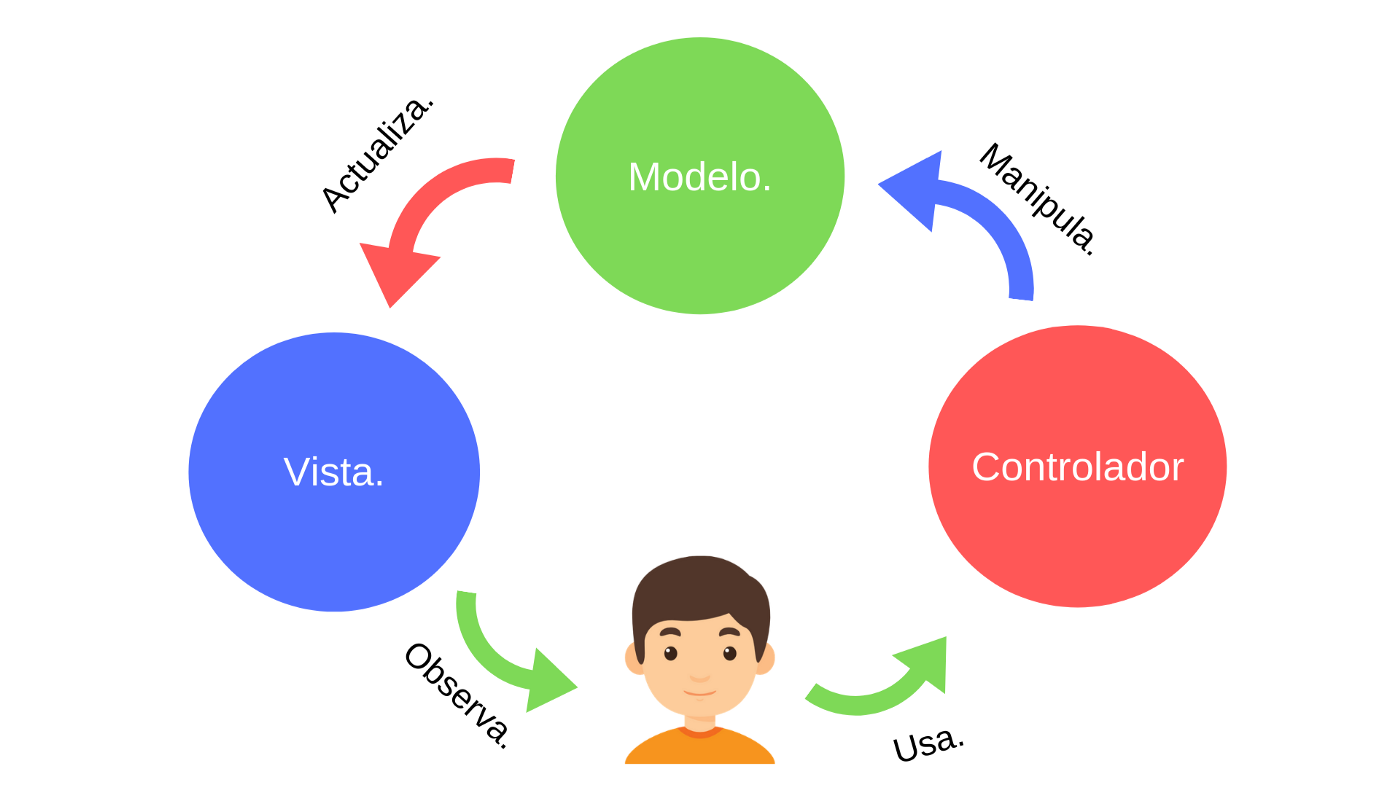
\includegraphics[width=10cm,height=10cm,keepaspectratio]{img/mvc.png}
    \caption{Imagen de flujo en MVC \cite{mvcImag}.}
    \label{fig:mv}
\end{figure}
\FloatBarrier

\subsection{Maestro-Esclavo}

Esta arquitectura se basa en un elemento maestro controla y se comunica con los esclavos, que hacen lo que le pida el maestro.

Esta arquitectura se utiliza en las \textit{Raspberries}, pero como el proyecto no es de gran escala, solo se utilizan componentes maestros.

\FloatBarrier
\begin{figure}[h]
    \centering
    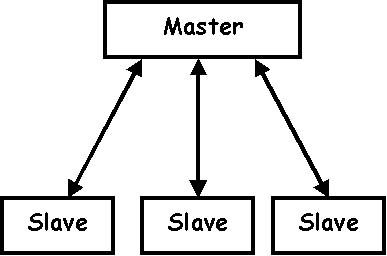
\includegraphics[width=7cm,height=7cm,keepaspectratio]{img/masterslave.jpg}
    \caption{Diagrama de maestro esclavo \cite{masterslaveimg}.}
    \label{fig:diagram_seceunce_guide}
\end{figure}
\FloatBarrier
\subsection{Arquitectura general}
En este apartado se describirá mediante un esquema, la arquitectura general del sistema enseñado el uso de la arquitectura modelo controlador y el uso del \textit{ORM SqlAlchemy} para la conexión con la base de datos.
\FloatBarrier
\begin{figure}[h]
    \centering
    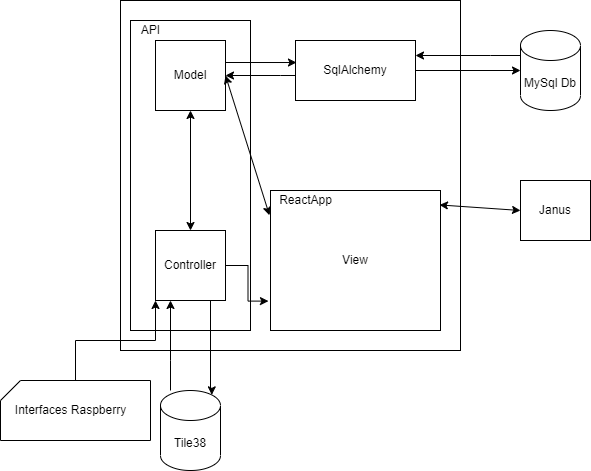
\includegraphics[width=10cm,height=10cm,keepaspectratio]{img/Esquema general del proyecto.drawio (1).png}
    \caption{Diagrama de la arquitectura general.}
    \label{fig:diagram_seceunce_guide}
\end{figure}
\FloatBarrier
\subsection{Diseño de paquetes}
En este subapartado se van a explicar la gestión de paquetes de la aplicación. La estructura general del proyecto es:
\FloatBarrier
\begin{figure}[h]
    \centering
    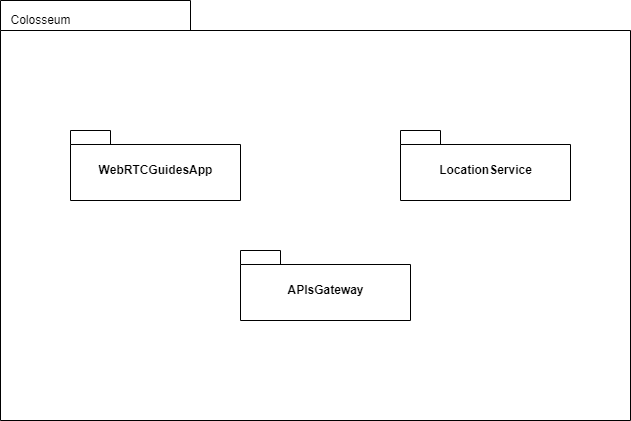
\includegraphics[width=10cm,height=10cm,keepaspectratio]{img/packetsGeneral.drawio (1).png}
    \caption{Paquetes de la aplicación.}
    \label{fig:diagram_seceunce_guide}
\end{figure}
\FloatBarrier
La descripción de cada uno de los paquetes es:
\begin{itemize}
    \item \textit{\textbf{WebRTCGuidesApp}}: Todo el código relacionado con la \textit{webapp} de \textit{React}.
    \item \textit{\textbf{APIsGateway}}: Todo el código relacionado con servicios de la \textit{API}, la base de datos, el servidor web de producción y \textit{Janus}.
    \item \textit{\textbf{LocationService}}: Todo el código relacionado con el servicio de la localización.
\end{itemize}
\FloatBarrier
\begin{figure}[h]
    \centering
    \includegraphics[width=12cm,height=12cm,keepaspectratio]{img/Diseño General depaquetes.drawio.png}
    \caption{Subpaquetes de la aplicación.}
    \label{fig:diagram_seceunce_guide}
\end{figure}
\FloatBarrier

\subsection{Diseño de componentes}
En este apartado se describe como los componentes de la \textit{webapp} interaccionan entre sí:
\FloatBarrier
\begin{figure}[h]
    \centering
    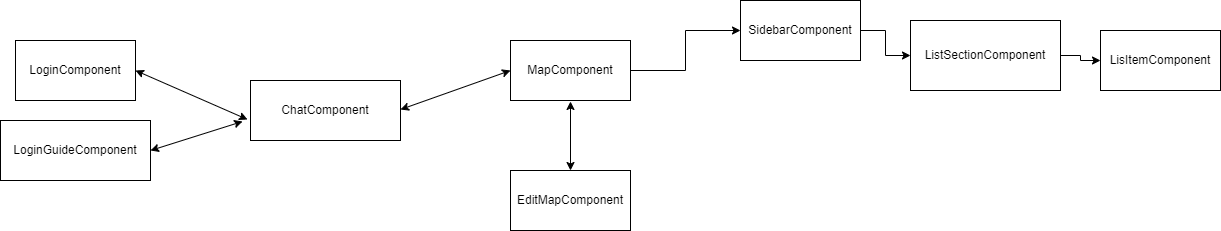
\includegraphics[width=12cm,height=12cm,keepaspectratio]{img/Diagrama de clases Colosseum.drawio.png}
    \caption{Diagrama de componentes de la \textit{webapp}: Interacción.}
    \label{fig:diagram_seceunce_guide}
\end{figure}
\FloatBarrier
\section{Diseño de interfaces}
Para el diseño de las páginas de la \textit{webapp}, se utilizó la herramienta \textit{Figma} para hacer unos bocetos iniciales de las paginas, pero se abandonó el proceso de diseño por falta de tiempo y se intentó adaptar a los diseños ya implementados de la página.

La aplicación web tiene 5 páginas bien diferenciadas siendo estas:
\begin{itemize}
    \item \textit{\textbf{Login}}
    \item \textit{\textbf{LoginGuide}}
    \item \textit{\textbf{Chat}}
    \item \textit{\textbf{Map}}
    \item \textit{\textbf{EditMap}}
\end{itemize}

Algunas imágenes de las interfaces de usuario son son:
\FloatBarrier
\begin{figure}[h]
    \centering
    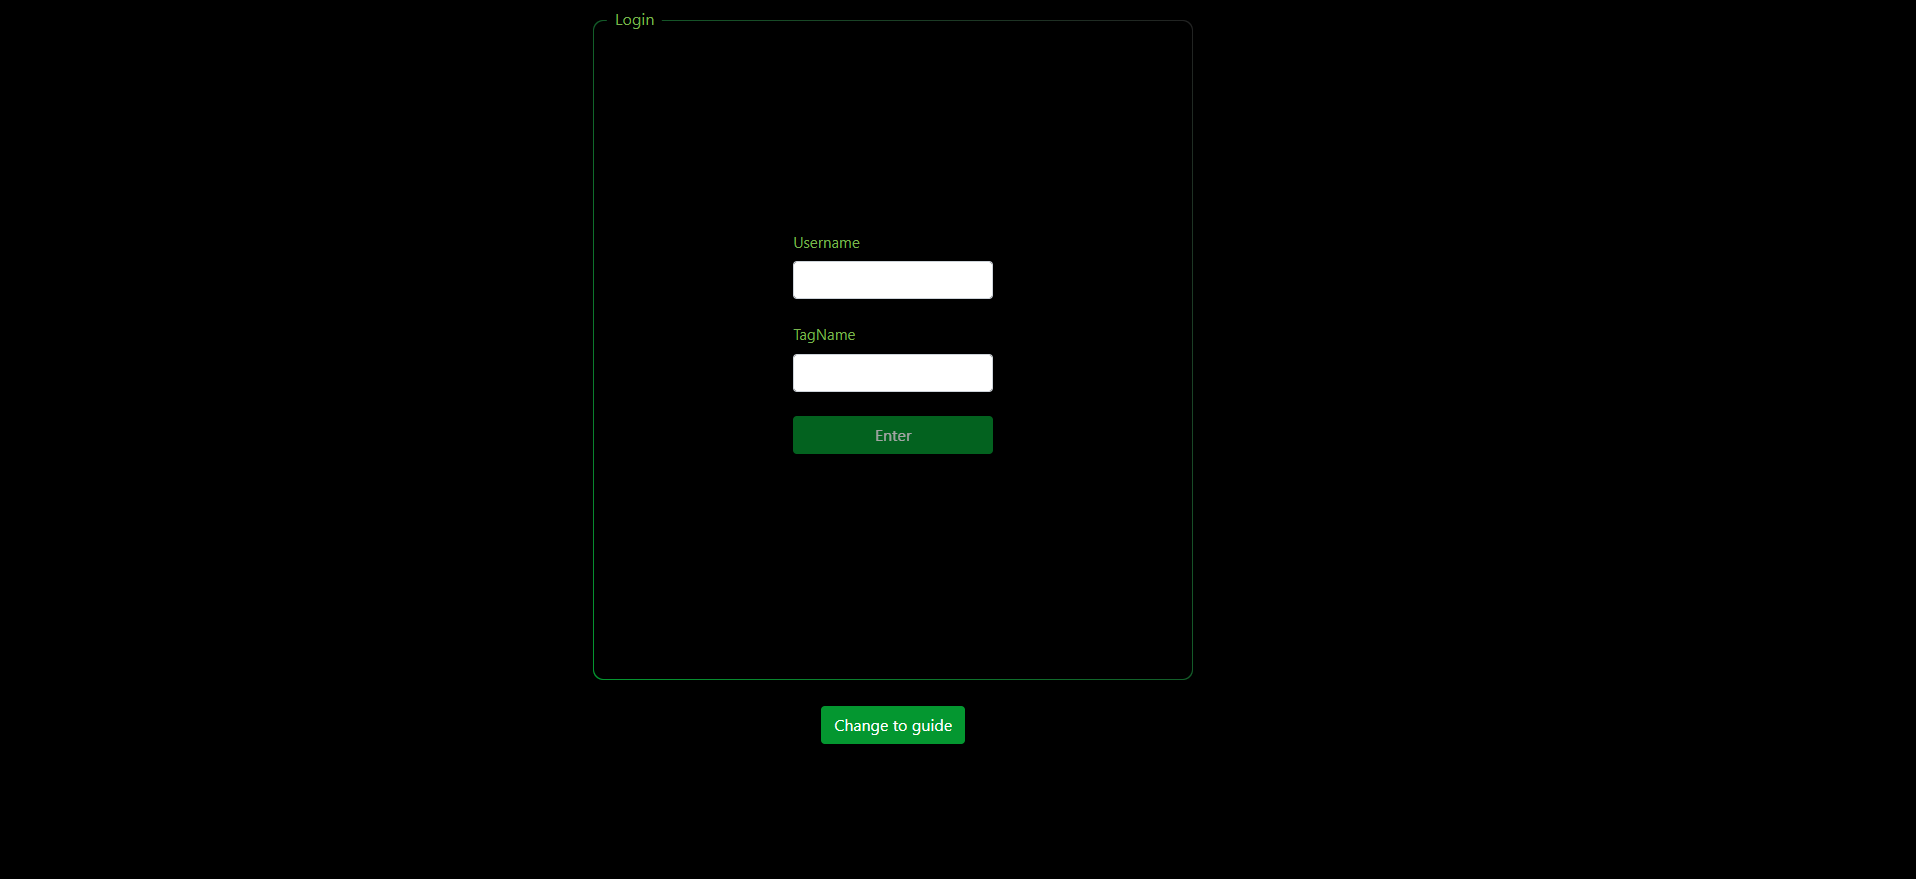
\includegraphics[width=12cm,height=12cm,keepaspectratio]{img/Login.png}
    \caption{Login del usuario.}
    \label{fig:Login del usuario}
\end{figure}
\FloatBarrier
\FloatBarrier
\begin{figure}[h]
    \centering
    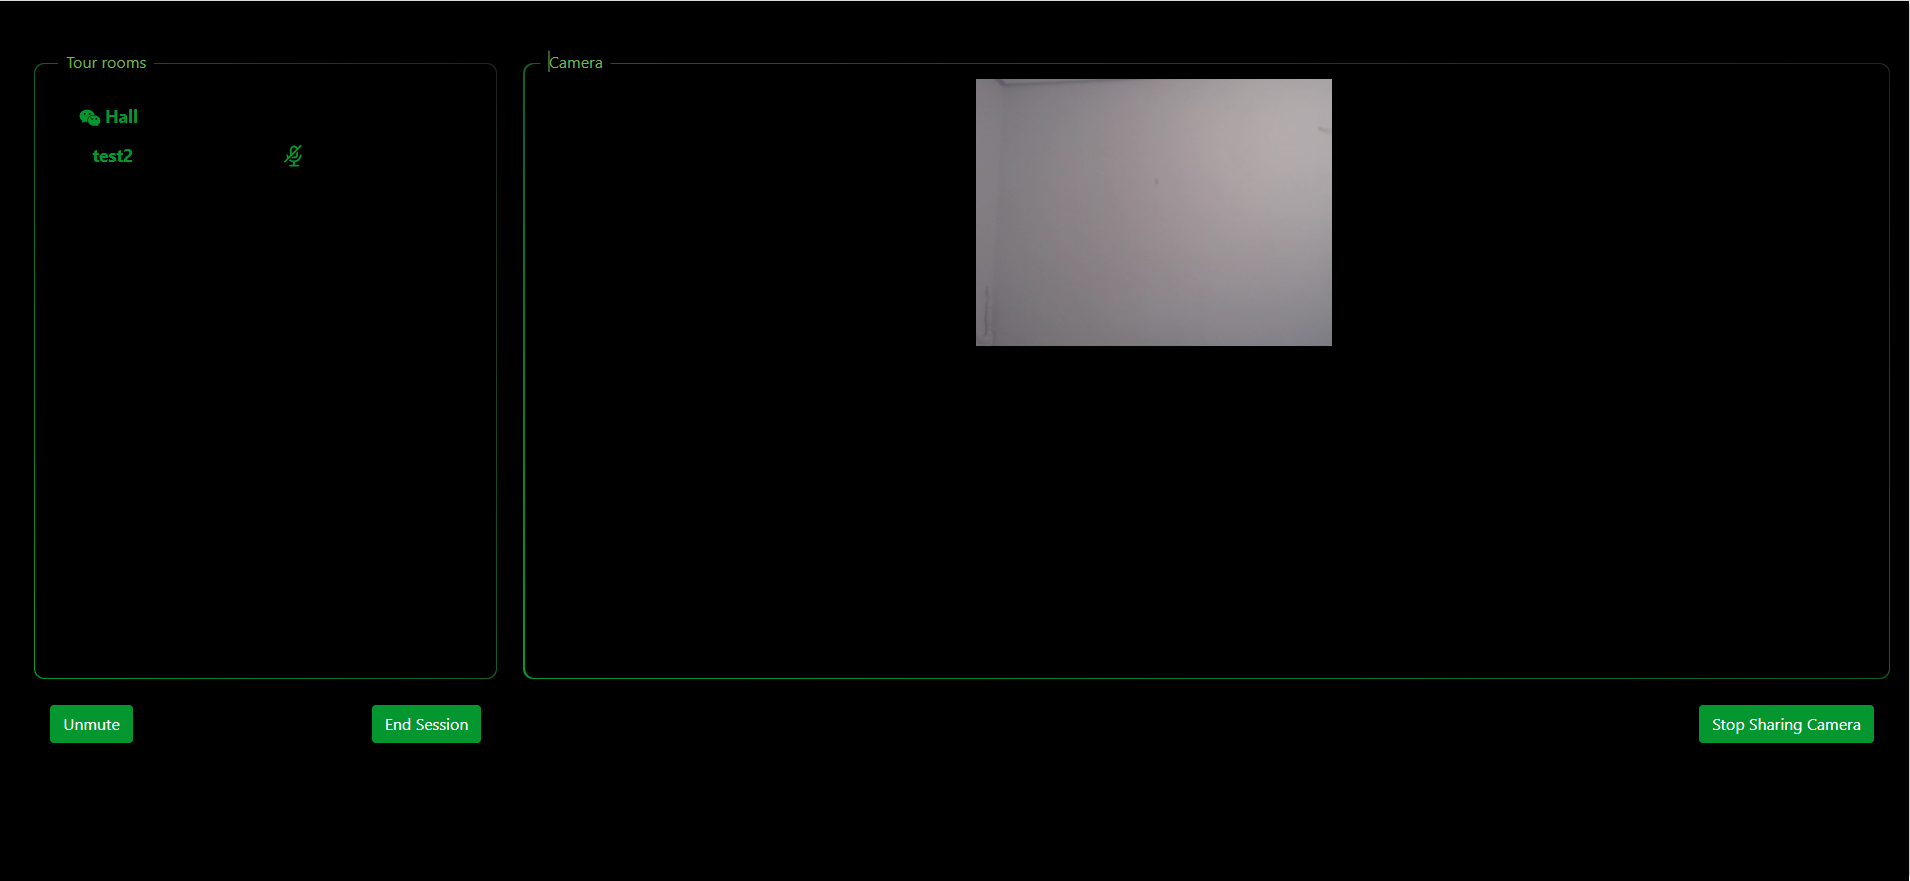
\includegraphics[width=12cm,height=12cm,keepaspectratio]{img/UserChatDesktop.png}
    \caption{Chat desde la vista del usuario.}
    \label{fig:Chat desde la vista del usuario}
\end{figure}
\FloatBarrier
\FloatBarrier
\begin{figure}[h]
    \centering
    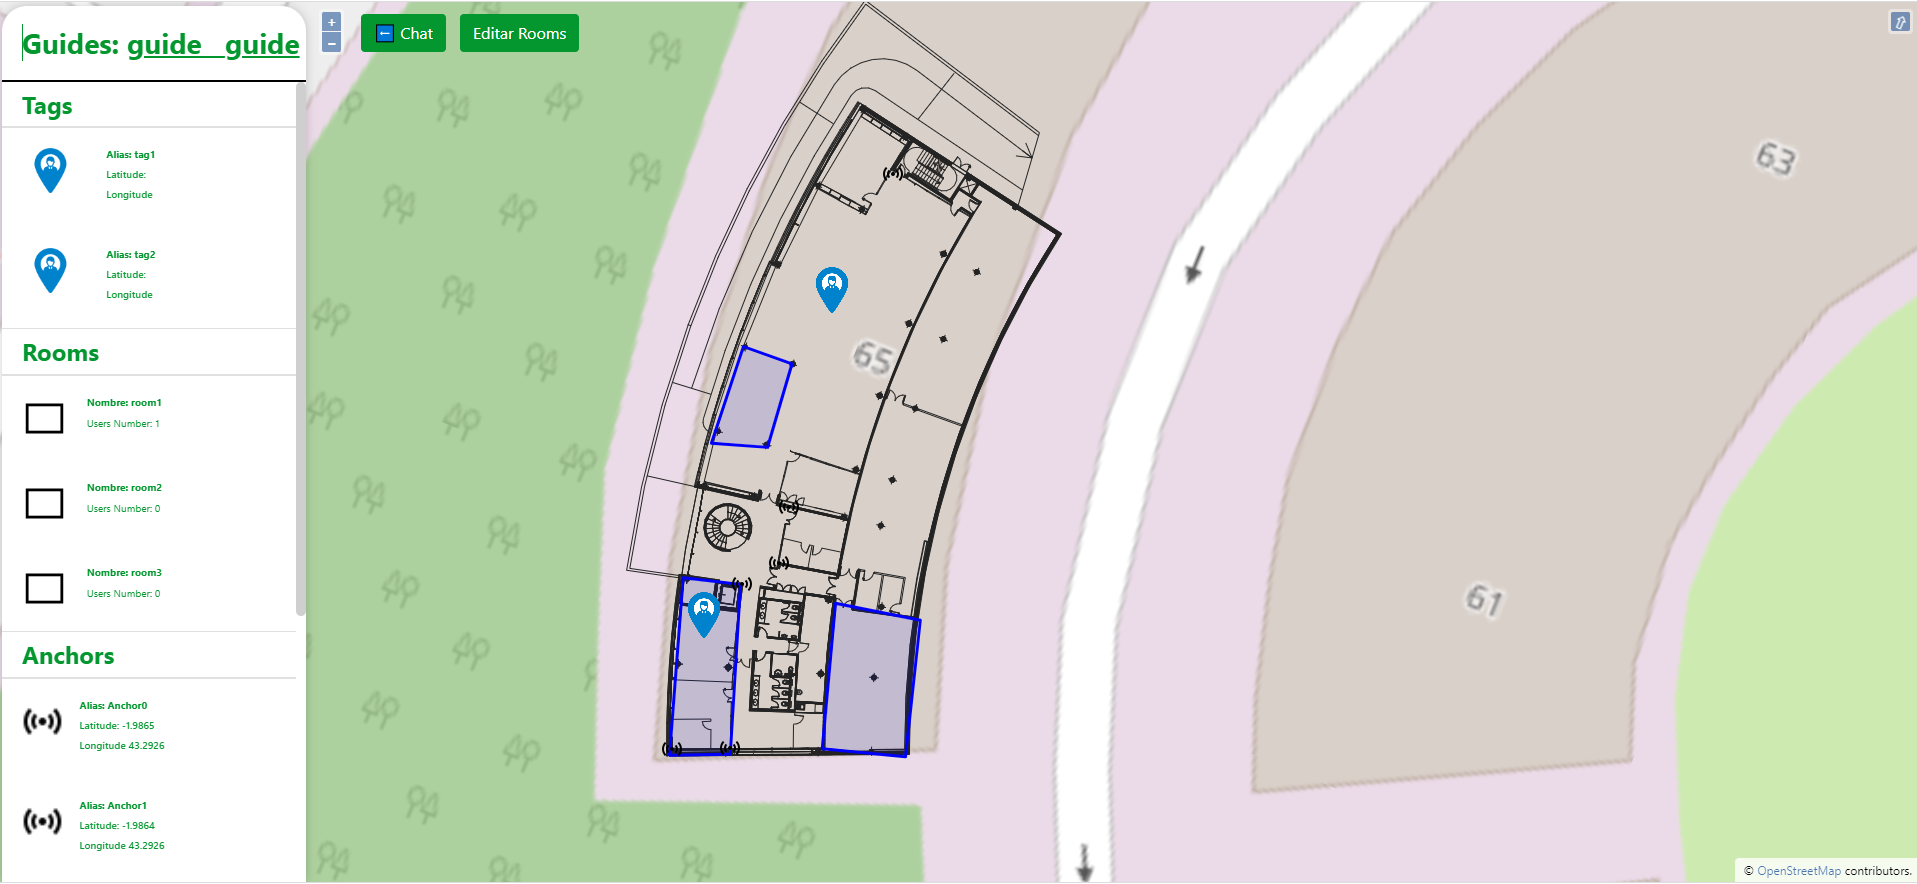
\includegraphics[width=12cm,height=12cm,keepaspectratio]{img/Map.png}
    \caption{Mapa del guía.}
    \label{fig:Mapa del guía}
\end{figure}
\FloatBarrier

Por otro lado el siguiente diagrama muestra el flujo de navegabilidad por las paginas de los usuarios:

\FloatBarrier
\begin{figure}[h]
    \centering
    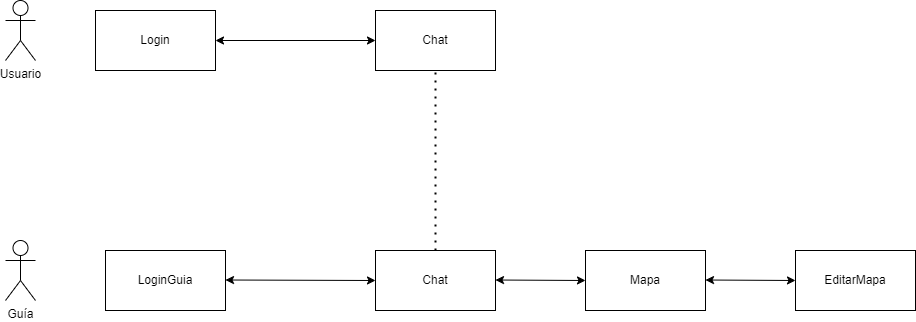
\includegraphics[width=12cm,height=12cm,keepaspectratio]{img/Flujo de navegabilidad.png}
    \caption{Diagrama de flujo de navegabilidad de los usuarios por las páginas.}
    \label{fig:Flujo de navegabilidad de los usuarios por las páginas}
\end{figure}
\FloatBarrier